\chapter{Testing}

Testing is an inseparable component of software development and is an integral part of the code writing process. In order to ensure the designed and implemented system works correctly and satisfies the requirements placed upon it, three different approaches to testing and verification were chosen: automated tests, manual tests and performance tests. This chapter describes the performed tests, the environments in which they were performed, and their outcomes along with derived conclusions.

\section{Automated Testing}
Automated tests for the application are written using the Spock framework, described in Chapter \ref{analysis:spock} \nameref{analysis:spock}. The Spock framework has a powerful mocking API, which is used in order to test application logic in isolation in the form of unit tests. Spock also provides support for easily implemented Data Driven and Interaction Based testing, both of which were used.

Where needed, automated Spock's Spring plugin is used in order to run integration tests, which are used for verification of logic that relies on the Spring Application Context to be loaded. For integration tests, an embedded H2\footnote{H2 Database Engine <\url{http://www.h2database.com/html/main.html}>} database is used, allowing for tests to easily be run automatically by continuous integration tools, without the need of supplying an external test database.

\section{Manual Testing}
Due to the nature of the system and the complexity of testing a distributed system, the sample implementation application, Chattr, was created to verify the proper behaviour of the system. Using this, a large part of the tests of the functionality of the system as a whole was done using manual tests, based on use-case scenarios. This section describes the test scenarios and the environment in which they were performed.

\subsection{Testing Environment} \label{test:test-env}
In order to approximate a distributed environment, the testing environment consists of two machines, on which the system is run, utilizing each machine to run multiple applications and Nodes. The deployment diagram of the system testing environment can be seen in Figure \ref{fig:test-deploy-dia}.

\begin{figure}[!ht]
	\centering
	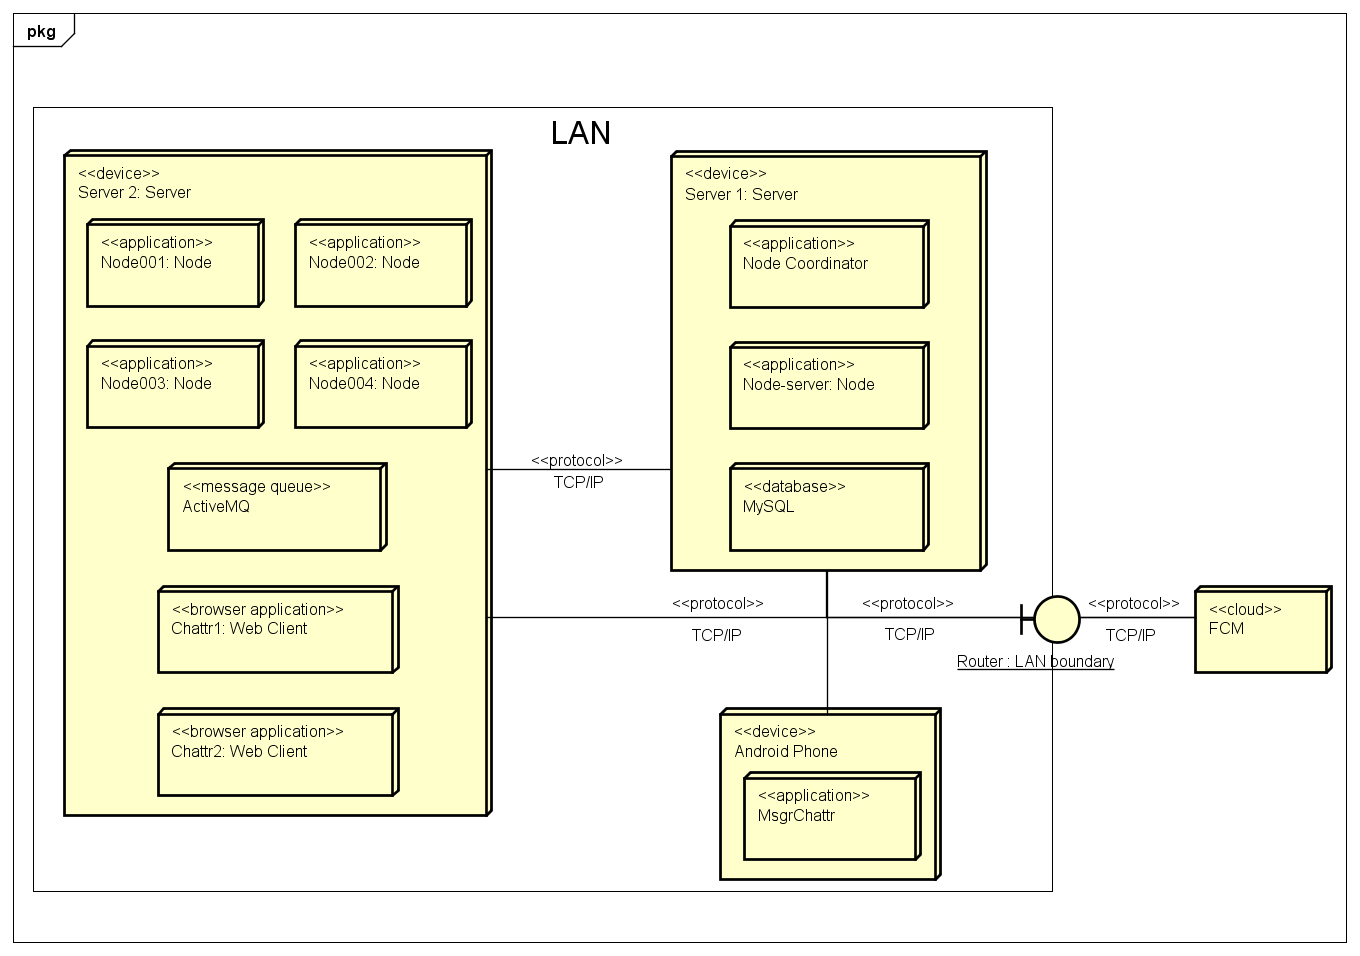
\includegraphics[width=1\textwidth]{figures/05_testing/test-deploy-dia}
    \caption{Deployment diagram of the testing environment}
    \label{fig:test-deploy-dia}
\end{figure}

The machine called \textit{Server2} runs four Node instances, an ActiveMQ instance and two instances of the Web client, Chattr. The second machine, called \textit{Server1}, runs a Node instance, the Node Coordinator, and a MySQL database. Both machines share the same Local Area Network (LAN), with an Android smart phone also connected to the same network. The LAN is connected to the internet, where the Firebase Cloud Messaging service resides in the cloud.

\subsubsection{Testing Environment Machine Specifications}
The hardware and operating system specifications of the two machines used in the testing environment are detailed in Table \ref{tab:test-hw}.

\begin{table}[!ht]
\begin{center}
\begin{tabularx}{\textwidth}{l|X|X|l}
\hline
\textbf{Machine} & \textbf{Operating System} & \textbf{CPU} & \textbf{RAM} \\
\hline
Server1 & Ubuntu Server 16.04 LTS x64 & Intel Core i5-7500T, 4 cores @ 2.7GHz & 8GB DDR3L 1600MHz \\
\hline
Server2 & Windows 10 Home x64 & Intel Core i7-3610QM, 4 cores @ 2.3GHz & 16GB DDR3 1600MHz \\
\hline
\end{tabularx}
\end{center}
\caption{Testing environment machine specifications}
\label{tab:test-hw}
\end{table}

\section{Performance Testing}
As the system is meant to support large-scale real-time applications, performance is critical. For the purposes of gauging the system's message throughput in different scenarios, a performance benchmark application was created. The \textit{PerformanceTester} application is a console application written in Groovy, which uses the \textit{Java-Client} library to communicate with the system.

This Section describes the performance tests performed, presents the obtained experimental data and uses it to formulate conclusions on the system's performance.

\subsection{Tests}
All tests were performed in the testing environment described in Section \ref{test:test-env} \nameref{test:test-env}, with messages being addressed to a user. This means the message goes through the following flow:

The message is sent to a Node, where it gets processed and pushed into the user message queue, from which another Node dequeues it, processes it, and as it is a message addressed for a user, unfolds the user into their devices, pushing the message into the devices respective message queues. After this, the Nodes that each of these devices is bound to dequeues the message and passes it to its client.

Every test was repeated four times in order to average out any abnormalities caused by other processes on the machines.

The precision of the time measurements is in milliseconds (ms).

\subsection{Test 1: Single Node, single client. 50 messages}
In this test, the system consist only of \textit{Node001}, running on the same machine as the PerformanceTester application. 

The PerformanceTester connects a single client to the Node and sends 50 messages addressed to itself. As all of the messages are sent almost simultaneously, with no delay between them, this test floods the system with a large number of messages at the same time.

\begin{table}[!ht]
\begin{center}
\begin{tabularx}{0.7\textwidth}{l|l}
\hline
\textbf{Measurement \#} & \textbf{Average message delivery time (ms)} \\
\hline
1 & 0.3\\
\hline
2 & 0.42\\
\hline
3 & 0.48\\
\hline
4 & 0.18\\
\hline
\end{tabularx}
\end{center}
\caption{Average message delivery time for Test 1}
\label{tab:test-perf1}
\end{table}

\begin{figure}[!ht]
	\centering
	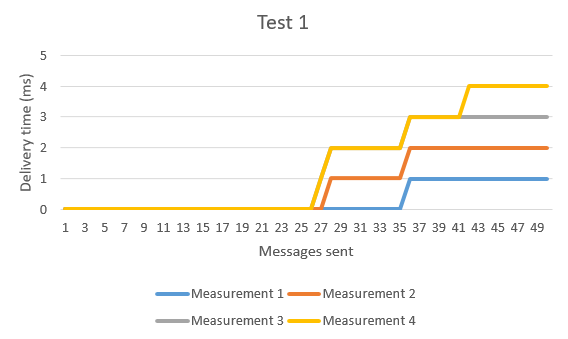
\includegraphics[width=0.7\textwidth]{figures/05_testing/test-perf1}
    \caption{Test 1: Delivery times}
    \label{fig:test-perf1}
\end{figure}

\subsection{Test 2: Single Node, single client. 200 messages}
The scenario for this test is the same as for Test 1, except this time 200 messages are sent simultaneously.

\begin{table}[!ht]
\begin{center}
\begin{tabularx}{0.7\textwidth}{l|l}
\hline
\textbf{Measurement \#} & \textbf{Average message delivery time (ms)} \\
\hline
1 & 1.205\\
\hline
2 & 1.125\\
\hline
3 & 1.105\\
\hline
4 & 1.32\\
\hline
\end{tabularx}
\end{center}
\caption{Average message delivery time for Test 2}
\label{tab:test-perf2}
\end{table}

\begin{figure}[!ht]
	\centering
	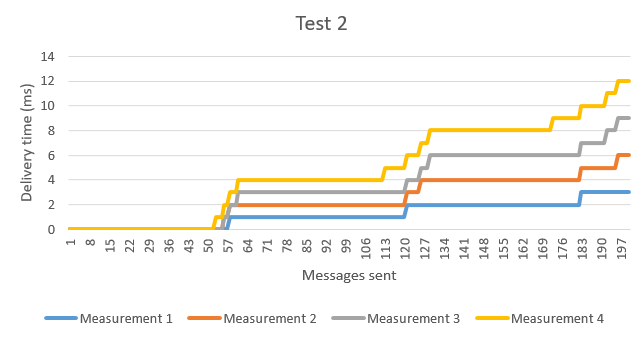
\includegraphics[width=0.7\textwidth]{figures/05_testing/test-perf2}
    \caption{Test 2: Delivery times}
    \label{fig:test-perf2}
\end{figure}

\clearpage

The data from Tests 1 and 2 shows a clear connection between the number of messages sent simultaneously and their delivery time. This is most likely due to the congestion of the websocket communication channel, as all messages are pushed into it at once with little to no spacing between them.

\subsection{Test 3: 4 Nodes, single machine. 50 messages}
The scenario for this test is similar to the scenarios in Tests 1 and 2, except now the \textit{Server2} machine is running four Nodes and the PerformanceTester is running a client for each. For every message to be sent, a random client is chosen and the message is sent as a broadcast to all the clients, including the sender. This effectively means that while 50 messages are sent out, 200 messages in total are received - 50 for each client.

\begin{table}[!ht]
\begin{center}
\begin{tabularx}{0.7\textwidth}{l|l}
\hline
\textbf{Measurement \#} & \textbf{Average message delivery time (ms)} \\
\hline
1 & 2.97\\
\hline
2 & 2.92\\
\hline
3 & 1.975\\
\hline
4 & 2.785\\
\hline
\end{tabularx}
\end{center}
\caption{Average message delivery time for Test 3}
\label{tab:test-perf3}
\end{table}

\begin{figure}[!ht]
	\centering
	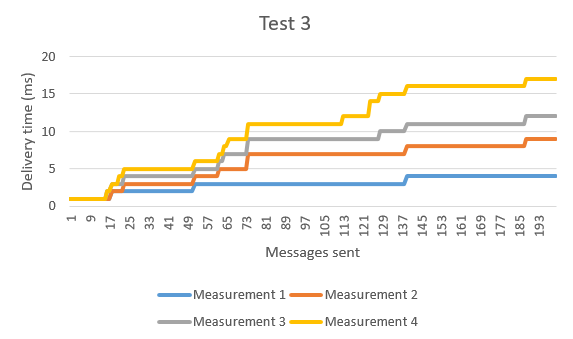
\includegraphics[width=0.7\textwidth]{figures/05_testing/test-perf3}
    \caption{Test 3: Delivery times}
    \label{fig:test-perf3}
\end{figure}

\subsection{Test 4: 5 Nodes, two machines. 50 messages}
The scenario for this test is almost the same as Test 3, except this time the \textit{Node-server} on machine \textit{Server1} is also running, scaling the system onto a second machine. As there are now 5 nodes, it also means 50 more messages need to be delivered, making it a total of 250 delivered messages.

\begin{table}[!ht]
\begin{center}
\begin{tabularx}{0.7\textwidth}{l|l}
\hline
\textbf{Measurement \#} & \textbf{Average message delivery time (ms)} \\
\hline
1 & 3.296\\
\hline
2 & 3.448\\
\hline
3 & 2.852\\
\hline
4 & 3.2\\
\hline
\end{tabularx}
\end{center}
\caption{Average message delivery time for Test 4}
\label{tab:test-perf4}
\end{table}

\begin{figure}[!ht]
	\centering
	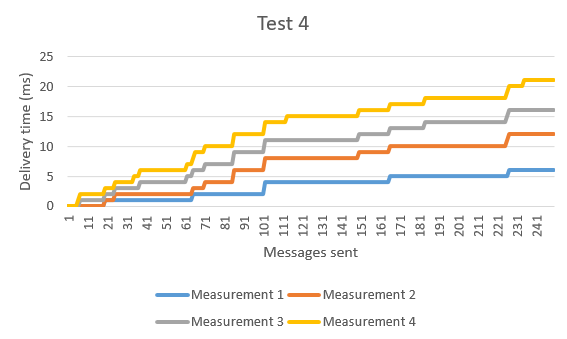
\includegraphics[width=0.7\textwidth]{figures/05_testing/test-perf4}
    \caption{Test 4: Delivery times}
    \label{fig:test-perf4}
\end{figure}

The data from Tests 3 and 4 continue to support the trend from Tests 1 and 2, where the larger the ammount of messages pushed through the communication channel at one time, the longer the message delivery time. However, for the same amount of delivered messages (200), we can see that Test 3 has higher average delivery time than Test 2. As Test 3 distributes the load among multiple Nodes, this further supports the hypothesis that the bottleneck that is being congested is the websocket connection, not the system itself.

\clearpage

\subsection{Test 5: Communication simulation. 50 messges, 20ms interval}
This scenario aims to simulate a real-time communication between two clients, with a two-way constant stream of data from one to the other and vice versa. One client is connected to Node \textit{Node001} on machine \textit{Server2} and the other to Node \textit{Node-server} on machine \textit{Server1}. The individual messages are separated with 20ms intervals, mimicking a real communication closer than the previous tests, which pushed all messages at once.

\begin{table}[!ht]
\begin{center}
\begin{tabularx}{0.7\textwidth}{l|l}
\hline
\textbf{Measurement \#} & \textbf{Average message delivery time (ms)} \\
\hline
1 & 0.42\\
\hline
2 & 0.42\\
\hline
3 & 0.32\\
\hline
4 & 0.22\\
\hline
\end{tabularx}
\end{center}
\caption{Average message delivery time for Test 5}
\label{tab:test-perf5}
\end{table}

\begin{figure}[!ht]
	\centering
	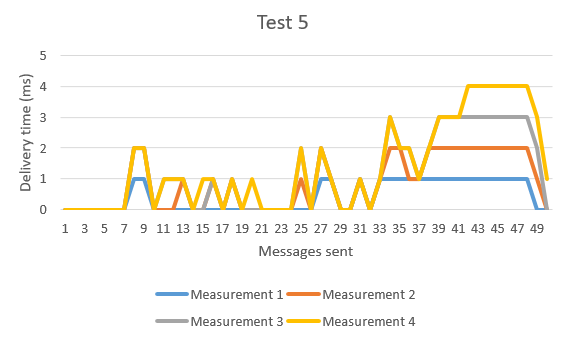
\includegraphics[width=0.7\textwidth]{figures/05_testing/test-perf5}
    \caption{Test 5: Delivery times}
    \label{fig:test-perf5}
\end{figure}

\clearpage

\subsection{Test 6: Communication simulation. 200 messages, 20ms interval}
This scenario is the same as the one in Test 5, except with 200 messages.

\begin{table}[!ht]
\begin{center}
\begin{tabularx}{0.7\textwidth}{l|l}
\hline
\textbf{Measurement \#} & \textbf{Average message delivery time (ms)} \\
\hline
1 & 2.17\\
\hline
2 & 2.19\\
\hline
3 & 1.21\\
\hline
4 & 1.47\\
\hline
\end{tabularx}
\end{center}
\caption{Average message delivery time for Test 6}
\label{tab:test-perf6}
\end{table}

\begin{figure}[!ht]
	\centering
	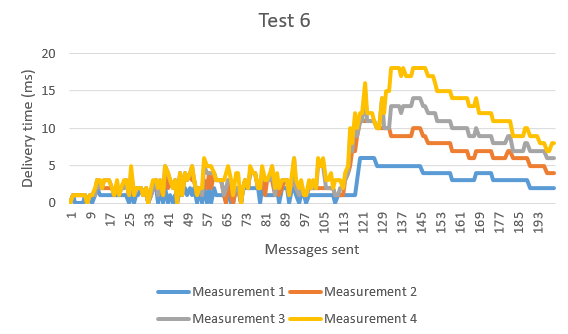
\includegraphics[width=0.7\textwidth]{figures/05_testing/test-perf6}
    \caption{Test 6: Delivery times}
    \label{fig:test-perf6}
\end{figure}

The data from Tests 5 and 6 immediately shows a drastic decrease in delivery time as congestion on the websockets is relieved and processing load is distributed over two machines. The times are higher than in Tests 1 and 2, but that is likely due to the fact that messages have to travel over the network to \textit{Node-server}, while Tests 1 and 2 were executed completely on a single machine.

\clearpage

\subsection{Test 7: Communication simulation. 200 messages, 100ms interval}
This scenario is the same as the one in Tests 5 and 6, except the interval between messages has been raised to 100ms to further free up the websocket channel. This scenario simulates a real-time application that sends ten messages per second.

\begin{table}[!ht]
\begin{center}
\begin{tabularx}{0.7\textwidth}{l|l}
\hline
\textbf{Measurement \#} & \textbf{Average message delivery time (ms)} \\
\hline
1 & 0.115\\
\hline
2 & 0.125\\
\hline
3 & 0.115\\
\hline
4 & 0.095\\
\hline
\end{tabularx}
\end{center}
\caption{Average message delivery time for Test 7}
\label{tab:test-perf7}
\end{table}

\begin{figure}[!ht]
	\centering
	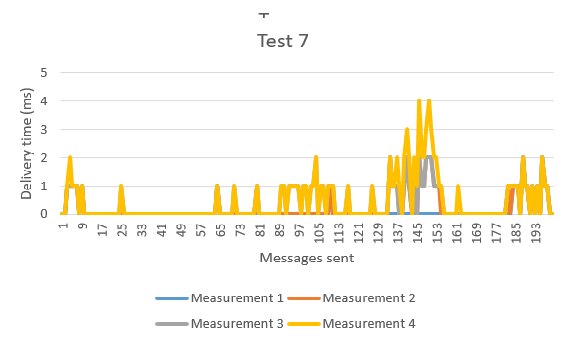
\includegraphics[width=0.8\textwidth]{figures/05_testing/test-perf7}
    \caption{Test 7: Delivery times}
    \label{fig:test-perf7}
\end{figure}

\subsection{Test 8: Communication simulation. 1000 messages, 100ms interval}
This scenario is the same as the one in Tests 7, but with 1000 messages.

\begin{table}[!ht]
\begin{center}
\begin{tabularx}{0.7\textwidth}{l|l}
\hline
\textbf{Measurement \#} & \textbf{Average message delivery time (ms)} \\
\hline
1 & 0.189\\
\hline
2 & 0.061\\
\hline
3 & 0.082\\
\hline
4 & 0.52\\
\hline
\end{tabularx}
\end{center}
\caption{Average message delivery time for Test 8}
\label{tab:test-perf8}
\end{table}

\begin{figure}[!ht]
	\centering
	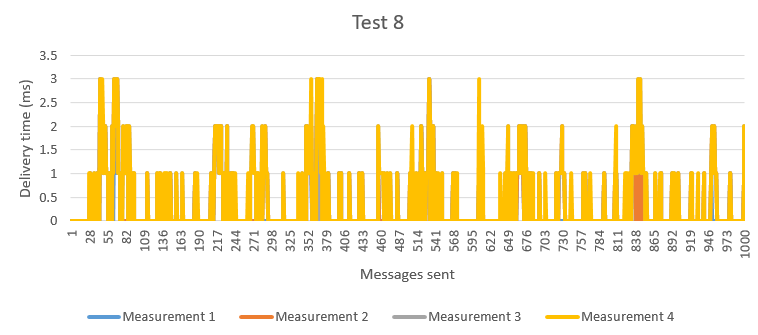
\includegraphics[width=0.9\textwidth]{figures/05_testing/test-perf8}
    \caption{Test 8: Delivery times}
    \label{fig:test-perf8}
\end{figure}

\subsection{Performance Test Conclusion}
The data from Tests 7 and 8 shows that most messages are delivered under 1ms, even with a large volume of messages. Combining this with the data from Tests 1 through 6, it can be assumed that the largest bottleneck of the system is the websocket channel between Nodes and clients and is based solely on connectivity.
